This chapter introduces our methodology and presents our experiment setup and results.
First of all, we introduce and justify the methods we use to evaluate agent performance in the Pac-Man environment.
We then show the results obtained using the chosen technique and analyze them, using the tools provided in our framework.

\section*{Evaluation in Reinforcement Learning}
\textbf{Evaluation} is a fundamental part of any machine learning project and reinforcement learning is not an exception to this rule.
The goal of evaluation in RL is analogous to that of supervised learning, in the sense that both are concerned with measuring how well a model \emph{generalizes}.

The aim of evaluation in RL is to measure the extent to which the acquired behaviour of the agent generalizes to the class of environment it learned in.
In other words, researchers try to certify if the agent learns meaningful \emph{skills} -- patterns in behaviour which are general enough to solve the problems they are developed to solve, even if presented from a new perspective.

In a similar manner, in supervised learning, models are evaluated based on their ability to accurately predict, estimate or classify previously unseen data -- their generalization ability.
A key difference between RL and its supervised counterpart is the latter's clearer methodology of dividing the dataset.
Experiments in supervised learning can and must split their data into specific subsets -- one for training and one for evaluation. In the RL setting, this separation is seldom possible.

Attempts to correct this overlap between training and evaluation in experimental RL is an active area of research.
One compelling paper concerning itself with this problem, published by OpenAI researchers, proposes building \emph{procedural generation} into environments \cite{procgen-paper}.
\clearpage

\section*{Setup and Methodology}
The evaluation \textbf{methodology} we chose for this thesis was used before across numerous RL studies, including in DeepMind's DQN and Double DQN works \cite{atari-dqn,ddqn-paper} and has been originally proposed in the Atari Learning Environment (ALE) paper \cite{ale-paper}, which was specifically developed to analyze agent perfromance in video game environments on the Atari 2600.
We follow the above guidelines closely, with a few exceptions.
For example, we will not be including including human performance in our benchmark.

To increase performance, we use a fixed frameskip $k$ inside the environment.
This multiplies number of environment steps the agent can advance per learning step, with only minimally impacting learning.
This technique\footnotemark{} has been proposed and used by the DeepMind team in the original DQN study \cite{atari-dqn}.
\footnotetext{DQN uses $k = 4$ for most games, except for Space Invaders which requires $k = 3$ because of an overlap with the period at which the projectiles blink \cite{atari-dqn}.}

We use \textbf{epsilon annealing} for the $\varepsilon$-greedy policies, another technique in the DQN standard.
The approach consists of linearly decreasing epsilon from $1$ to a predetermined lower bound, usually $10\%$ or $5\%$, to ensure non-zero exploration probability over the entire training run.
The role of this is to ensure that the agent does not get stuck in a local optimum, as well as to prevent overfitting to the environment.
If we allow the exploration coefficient to go all the way to zero, we risk having an agent learn a pattern that is inefficient or even counterproductive and would have no way of stopping it short of restarting the training run.

Our experiment setup starts from well-established standards in order to find ways to tweak them.
The implementation we use for our task environment is \texttt{MsPacman-v4}, provided by OpenAI within the \texttt{gym} package.
The base name of the game is \texttt{MsPacman}, designating the Atari 2600 version of Pac-Man.
The package offers multiple variables which control stochasticity of the environment.
An environment labeled \texttt{Deterministic} will have a fixed frameskip, set to $k = 4$ in our case.
The label \texttt{v4} indicates that the agent action is not repeated (besides the frame-skipping aspect), in contrast to \texttt{v0} which specifies a 25\% chance the previous action is repeated.

Our choice of hyperparameters is illustrated in Table \ref{tab:our-hyperparameters}.
Most hyperparameters are kept unchaged from the original papers they have been proposed in \cite{atari-dqn, per-paper}.
Our exploration coefficient $\varepsilon$ is chosen such that the lower bound is reached after 90\% of the training is done.

\begin{table}
    \centering
        \begin{tabular}{ll}
            \textbf{Name}                  & \textbf{Value}   \\
            learning rate $\alpha$             & 1e-4    \\
            discount factor $\gamma$           & 0.99    \\
            initial $\varepsilon$              & 1       \\
            terminal $\varepsilon$             & 0.05    \\
            $\varepsilon$ decay                & 8.62e-5 \\
            batch size                         & 32      \\
            swap frequency (number of steps)   & 1000    \\
            PER $\alpha$                       & 0.6     \\
            PER $\epsilon$                     & 0.01    \\
        \end{tabular}%
        \caption{Hyperparameters used to train our agent models.}
    \label{tab:our-hyperparameters}
\end{table}

\section*{Results}
We train each agent for $122,240$ episodes, without keeping a count of environment steps (i.e., actions played inside the emulator) or frames seen, so the exact number of steps can vary between training runs.
Other studies design their training routines to run for a finite number of steps.
However, in our design, one episode produces one data point. We have chosen not to follow this guideline as it would be easier to stop when we have gathered exactly the same amount of data on each run.
Each training job ran for 10-15 hours of wall clock time, depending on the complexity of each algorithm.

We run four algortihms in this setup: \texttt{dqn}, \texttt{doubledqn}, \texttt{per} and \texttt{doubleper}.
Each algorithm was covered separately in Section \ref{section:implementation}.
The results of their training runs are represented in Figure \ref{fig:training-results}.
The plot refects a limited window of each agent's learning ability and hints to potential drawbacks and advantages of each technique in Pac-Man.

\begin{figure}[h]
    \centering
    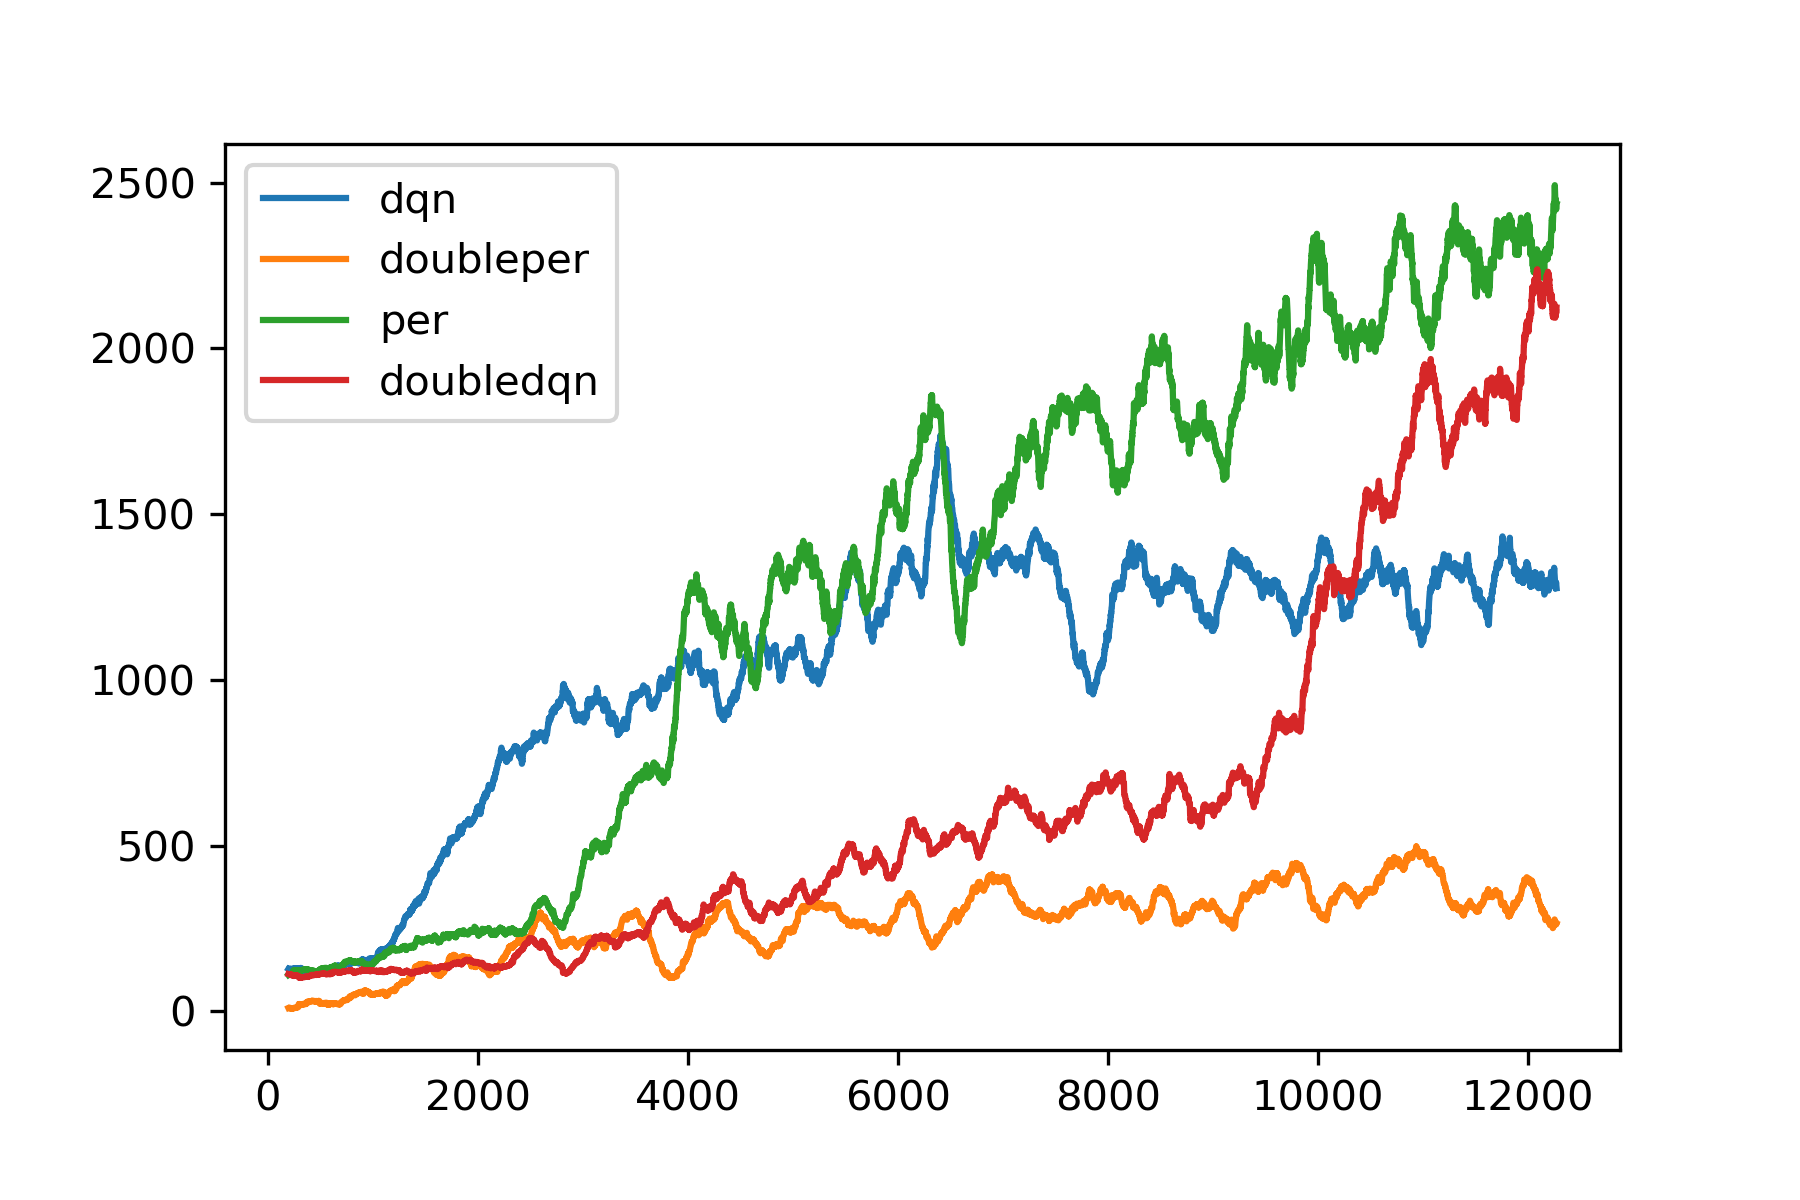
\includegraphics[width=0.9\textwidth]{training-comparison-plot.png}
    \caption{A performance comparison during agent \textbf{training}, showing each algortihm in a different color. The x-axis shows the episode number while the y-axis represents the obtained score.}
    \label{fig:training-results}
\end{figure}

We observe that, from the training perspective, the most performant two methods are double Q-learning and PER, which are able to learn steadily and reliably over the course of the experiment and appear to hold onto this growth trend towards the end of their respective runs.
This is an expected result as these two techniques are frequently cited as a significant improvement over the baseline DQN.
The unexpected result is prioritized double Q-learning, the hybridization of the above two best performers (labeled \texttt{doubleper} and presented in yellow in Figure \ref{fig:training-results}) does not score above the DQN baseline (in blue) -- it in fact manages to score lower, showing little to no improvement.
Some agents do fail to improve at some games using this technique, as attested by the benchmark provided by Schaul et al. \cite{per-paper}.
The two components of the hybrid interfere with each other and result in a weaker agent.
We hypothesize that this underperformance is due to the harsh memory contstraints the agent was operating under.
Small buffer sizes could hinder the algorithm's ability to gather large enough sample before starting to forget vital information, despite it being properly prioritized.
Also notable is that double Q-learning was slower to generalize than the baseline.
This could hint that \texttt{doubleper} simply did not have a long enough run to start properly generalizing.

\begin{table}
    \centering
        \begin{tabular}{ll}
            \textbf{Agent / Algorithm} & \textbf{Average score (over 2000 episodes)}   \\
            Random agent               & 243.3 \\
            Baseline DQN               & 1532.2 \\
            Double DQN                 & 2280.5 \\
            \textbf{PER}               & \textbf{2953} \\
            Double PER                 & 646.35 \\
        \end{tabular}%
        \caption{Results of agent \textbf{evaluation}. Each agent has been run for 2000 full episodes.}
    \label{tab:evaluation-results}
\end{table}

In Table \ref{tab:evaluation-results} we present the results of evaluation.
The evaluation is done by taking snapshots of final agent states (i.e., the state of the neural networks), \emph{unchaged} from the end of training.
The agents do not learn from new experiences during evaluation.

Other training snapshots were availabile to us as samples for evaluation.
However, we considered that hand-picking data would be unfair and would result in introducing bias from outliers, for example if we accidentally hand-picked performant snapshots which happened in local optima.

We remark that the ranking stays the same, being a natural continuation of the trend demonstrated during training, with double DQN and PER on top of it.
The new aspect in the evaluation table is the inclusion of a random agent, to serve as comparison.
Judging by the difference from random noise, we can conclude that the agents succesfully learn, with even the underperforming algorithm achieving  2-3 times the score of the random agent. The first ranking algorithm scores 12 times above the random agent and almost 2 times the DQN baseline.